%%
%% Copyright 2007, 2008, 2009 Elsevier Ltd
%%
%% This file is part of the 'Elsarticle Bundle'.
%% ---------------------------------------------
%%
%% It may be distributed under the conditions of the LaTeX Project Public
%% License, either version 1.2 of this license or (at your option) any
%% later version.  The latest version of this license is in
%%    http://www.latex-project.org/lppl.txt
%% and version 1.2 or later is part of all distributions of LaTeX
%% version 1999/12/01 or later.
%%
%% The list of all files belonging to the 'Elsarticle Bundle' is
%% given in the file `manifest.txt'.
%%

%% Template article for Elsevier's document class `elsarticle'
%% with numbered style bibliographic references
%% SP 2008/03/01
%%
%%
%%
%% $Id: elsarticle-template-num.tex 4 2009-10-24 08:22:58Z rishi $
%%
%%
\documentclass[preprint,10pt,5p]{elsarticle}
%% Use the option review to obtain double line spacing
%% \documentclass[preprint,review,12pt]{elsarticle}

%% Use the options 1p,twocolumn; 3p; 3p,twocolumn; 5p; or 5p,twocolumn
%% for a journal layout:
%% \documentclass[final,1p,times]{elsarticle}
%% \documentclass[final,1p,times,twocolumn]{elsarticle}
%% \documentclass[final,3p,times]{elsarticle}
%% \documentclass[final,3p,times,twocolumn]{elsarticle}
%% \documentclass[final,5p,times]{elsarticle}
%% \documentclass[final,5p,times,twocolumn]{elsarticle}

\usepackage{verbatim}
\usepackage{float}
%% if you use PostScript figures in your article
%% use the graphics package for simple commands
%% \usepackage{graphics}
%% or use the graphicx package for more complicated commands
%% \usepackage{graphicx}
%% or use the epsfig package if you prefer to use the old commands
%% \usepackage{epsfig}

%% The amssymb package provides various useful mathematical symbols
\usepackage{amssymb}
%% The amsthm package provides extended theorem environments
%% \usepackage{amsthm}

%% The lineno packages adds line numbers. Start line numbering with
%% \begin{linenumbers}, end it with \end{linenumbers}. Or switch it on
%% for the whole article with \linenumbers after \end{frontmatter}.
%% \usepackage{lineno}

%% natbib.sty is loaded by default. However, natbib options can be
%% provided with \biboptions{...} command. Following options are
%% valid:

%%   round  -  round parentheses are used (default)
%%   square -  square brackets are used   [option]
%%   curly  -  curly braces are used      {option}
%%   angle  -  angle brackets are used    <option>
%%   semicolon  -  multiple citations separated by semi-colon
%%   colon  - same as semicolon, an earlier confusion
%%   comma  -  separated by comma
%%   numbers-  selects numerical citations
%%   super  -  numerical citations as superscripts
%%   sort   -  sorts multiple citations according to order in ref. list
%%   sort&compress   -  like sort, but also compresses numerical citations
%%   compress - compresses without sorting
%%
%% \biboptions{comma,round}

% \biboptions{}


\journal{University of Melbourne}

\begin{document}

\begin{frontmatter}

\title{Next Generation Security for IoT in Post Quantum Era}

%%\tnotetext[label0]{This is only an example}

 
\author[label1]{Jigar Thakkar}
\address[label1]{School of Computing and Information Systems,The University of Melbourne, Australia, thakkarj@student.unimelb.edu.au}
%%\address[label2]{Address Two\fnref{label4}}

%%\cortext[cor1]{I am corresponding author}
%%\fntext[label3]{I also want to inform about\ldots}
%%\fntext[label4]{Small city}

%%\ead{author.one@mail.com}
%%\ead[url]{author-one-homepage.com}

\author[label2]{Priyalakshmi Gnanasekaran}
\address[label2]{School of Computing and Information Systems,The University of Melbourne, Australia, pgnanasekara@student.unimelb.edu.au}
%%\ead{pgnanasekara@student.unimelb.edu.au}

\author[label3]{Ge Yao}
\address[label3]{School of Computing and Information Systems,The University of Melbourne, Australia, gyao1@student.unimelb.edu.au}
%%\ead{gyao1@student.unimelb.edu.au}

\begin{abstract}
Internet of Things (IoT) is developing rapidly. As more and more smart devices being connected into network, the security problem has become the primary concern. In the past years, many cryptography based security solutions are proposed in literature. But the building blocks of these solutions are threatened by the arrival of quantum computing era. In this research, we study the cryptographic primitives that are suitable for the resource constrained IoT applications and also strong enough to resist the destructive power of quantum computers. We identify that lattice based cryptography and symmetric key cryptography are among the most simple and efficient algorithms among all the post quantum cryptographic primitives. We then explore the authentication problem in RFID based IoT application and discuss the stream cipher based authentication schemes.  

\end{abstract}

\begin{keyword}
%% keywords here, in the form: keyword \sep keyword
Internet of things \sep Post-quantum cryptography \sep Lattice based cryptography \sep Stream cipher \sep Authentication
%% MSC codes here, in the form: \MSC code \sep code
%% or \MSC[2008] code \sep code (2000 is the default)
\end{keyword}

\end{frontmatter}

%%
%% Start line numbering here if you want
%%
% \linenumbers

%% main text
\section{Introduction}
\noindent During the last three decades, connecting computers was a major focus, which becomes a global network of computers - the Internet. The Internet has enabled us to do all kinds of jobs which was just a science fiction three decades ago that included activities like group video chatting, www and cryptocurrency. Next revolution started by shaping the network of devices which included wireless sensors, RFIDs and whats more - the Internet of Things (IoT) thus came into being. 

For instance, imagine one day in the future when your car not only drives automatically, but also detects the surroundings, downloads all the latest traffic information of that area and chooses the best route to navigate you to office from your home. After dropping you at office, it will find parking space by itself, and if any maintenance is needed it will order parts spontaneously and go to the manufacturer for repair by itself.\cite{gerla2014internet} By the time, you finish your work in the evening, your smartwatch or wristband measures your body temperature and send it to smart home/automatic temperature control system, so that it starts maintaining the temperature. When you arrive and stay at home, your home will know in which part of the home you are and what activity you are doing. Lights will start turning on/ off as you move\cite{han2010smart}. There will be refrigerators which will show you the items in it and the  sophisticated algorithms will recommend a list of recipes which you can prepare from those items.Probably it should also be able to preorder the items in case it is running out, and smart internet enabled drones delivers it at your doorstep \cite{helal2005gator} \cite{zhou2014unmanned}. Apparently everything will be computerised and technologically sophisticated.

IoT not only makes human life easier but also healthier and safer. Smart pacemaker directly sends data of heart to the doctor/or some smart AI system, so that in case of emergency autonomous ambulance immediately takes the patient to the nearest hospital\cite{hernandez2001real}. IoT is not only smart but also efficient, and this is not in the future but it is already the present.According to estimate, IoT will have more than 30 billion internet connected devices before 2020. If we consider 7 billion population in the world, more than 4 devices will be owned by a single person \cite{atzori2010internet}. A huge chunk of this devices are currently used in industries.For example, Australia's largest independent oil and gas company-Woodside has already deployed 200,000 smart internet-connected sensors for plant monitoring in Perth, Western Australia. IoT is not just helping to manage industries but making them more productive and safer \cite{Bloede2015}.

But this all shiny promises of IoT turns dark when it gets hacked. Security is becoming major issues in IoT.If some malicious blackhat criminals hacks your car along with you inside then he can demand or force you to pay a huge ransom inorder to be harmless.Government can even start spying you by your smart home. What can be more dangerous than your body implanted device like pacemaker getting hacked? Industries can be sabotaged in the same way, and this has already happened. Germany recently banned smart doll which was spying, the DDoS attack happened by the network of IP cameras which was used as IoT botnet. Attacks by using IoT devices are much more disastrous than an attack on your computer because this can harm you physically, like bad robots of the Hollywood movies.

Security is challenging for IoT because it is a heterogeneous network. One of the biggest challenges is to ensure the security of small devices with limited capabilities and resources. The majority of these devices are embedded in the system with few MB of RAM and limited storage capabilities. The most common example is Raspberry Pi. Except for the limited resource, the nature of the device itself can be a problem. For example, some devices are custom designed which makes it is difficult to continue after-sales maintenance work once it is put to use. And some devices are hard to be replaced if they are installed in some remote areas like in space or inside human body. Moreover, cryptographic algorithms also have a limited lifespan, like RSA was hard to break before 10 years even with 512-bit key size but nowadays the standard has come to 2048 bit. 

With the conventional cryptographic algorithm which is present till date, we can protect our devices only to an extent. However, when the quantum computing era, cryptography will face dramatic changes. The security of the modern cryptographic algorithm is built on hard mathematical problems. For example, RSA is based on the integer factorization problem and RSA problem; ECC relies on the elliptic-curve discrete logarithm problem. But these can be easily broken down by the quantum computers. The work of Proos and Zalka shows that using 4096 qubit quantum computer and Shor's algorithm, RSA - 2048 bit can be broken \cite{Beckman1996}. Making key size larger is not the solution of this problem as computation power of quantum computers doubles by adding each new qubit, countering this we have to double RSA key size on each qubit.So it is clear that larger key size is an issue here for limited resources of IoT. Now comes the need to design strong and efficient algorithm to protect the heterogeneous IoT. 

In our research, we are considering the security solutions of IoT both for now and for the quantum age. First, we have studied algorithms proposed against quantum computers, which are collectively referred to as post-quantum cryptography. Several algorithms are believed to resist classical computers and quantum computers \cite{bernstein2009}, namely lattice based, hash based, multivariate, code based, super singular elliptic curve isogeny and symmetric key quantum resistance algorithm \cite{gabriel2013}. Our research mainly focuses on lattice based cryptography and symmetric key cryptography as they are considered as the most simple and efficient quantum resistance algorithms. Then we take RFID based IoT as an example and do further research on how to exploit cryptographic primitives to solve authentication problem in resource constrained IoT environment.

\section{Lattice based Cryptography}
\noindent Lattice based cryptography provides great promise for very strong security which is based on worst case hardness with efficient and simple implementation. The backbone of lattice based cryptography is hard mathematical problems like shortest vector problem, closest vector problem, bounded distance decoding etc wherein the public key encryption is built on these computational difficulties.

In the year 1995, Ajtai and Dwork have explained a lattice-based public key cryptosystem which has average case-worst case equivalence. Though it was only theoretical milestone and couldn’t be implemented practically. In 1996 Halevi,Goldwasser and Goldreich proposed a practically applicable lattice-based cryptosystem, after being motivated by the work of Dwork and Ajtai. The proposed system of GGH cryptosystem was fast, but then it needs large megabyte-size public keys to be secure while simultaneously, Hoffstein  was developing a ring-based cryptosystem known as NTRU that only requires RSA-sized keys. It has been lately indicated that NTRU can be explained by the terms of a special class of lattices which is closely related to the GGH system. Thus, lattice based cryptography includes approaches such as Ring-Learning with Errors, Learning with Errors, Ring-Learning with Errors, the Ring Learning with Errors Key Exchange and Ring-Learning with Errors, the older NTRU or GGH encryption schemes. Few of these approaches like NTRU encryption have been studied for several years without anyone finding a feasible attack whereas other approaches like the Ring-LWE algorithms have proofs that their security can be applied to a worst-case problem \cite{hoffstein2008introduction}.

A lattice can be defined as a set of points with a space of $n$-dimension as illustrated in Figure 1. It is considered that for a set of given $n$ linearly independent vectors. The lattice is generated by the set of vectors where $n$ linearly independent vectors $b_1,…, b_n$ are given which forms the basis of the lattice.
$$\zeta (b_1, ..., b_n)=\{\sum_{i=1}^{n} x_ib_i : x_i \in Z \} $$

\begin{figure}[H]
\centering
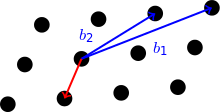
\includegraphics[width=0.3\textwidth]{Lattice.png}
\caption{Lattice}
\end{figure}

For example, in the above figure if we consider the shortest vector problem, we need to find the shortest distance vector for the two vectors $b1$ and $b2$ which are indicated by blue lines. Then red line is the shortest vector which we can find and this is really a very hard mathematical problem when it comes to 500-dimensional lattice. It is interesting that in $r$-approximate SVP for $r=poly(n)$, the SVP algorithm runs in time runs in time $2^n$. Also, it is not considered as the NP-hard problem. The possible poly-time algorithm solves for $r=2^{nloglogn/logn}$ \cite{du2015}. Lattice based cryptography provides the possibility of faster encryption and decryption algorithms. For example, let n be the number of bits in the below given problem:
\begin{itemize}
  \item $n$ =  number of bits in an RSA modulus $pq$
  \item $n$ =  number of bits in a prime p for ECC in $E(Fp)$
  \item $n$ = (dimension of a lattice L) $x$ ($#$ of bits in a coordinate)
\end{itemize}

Using various methods for encryption/decryption it takes $O (n^2 log n)$ steps for RSA and ECC whereas $O (n log n)$ steps for lattice-based cryptosystems which makes it more efficient. For learning with error problems, the practical implementation will be to distinguish noisy inner products from the uniform lattices \cite{hoffstein2008introduction}.
$$ a_1, b_1 = \langle a_1,s \rangle+e_1$$
$$ a_2, b_2 = \langle a_2,s \rangle+e_2$$
$$ 
 \Bigg(
  \begin{tabular}{c}
  ...\\
  
  A^t\\
  ...\\
  \end{tabular} \Bigg),\Bigg(
  \begin{tabular}{c}
  ...\\
  
  b\\
  ...\\
  \end{tabular} \Bigg)= A^ts+e
$$

where the generator matrix can be given as:
$$\zeta(A)=\{z\in Z^m : \exists s.z \equiv A^ts mod q $$

By applying it practically in case of Alice and Bob, message encryption, it can be illustrated in the picture as given below:

\begin{figure}[H]
\centering
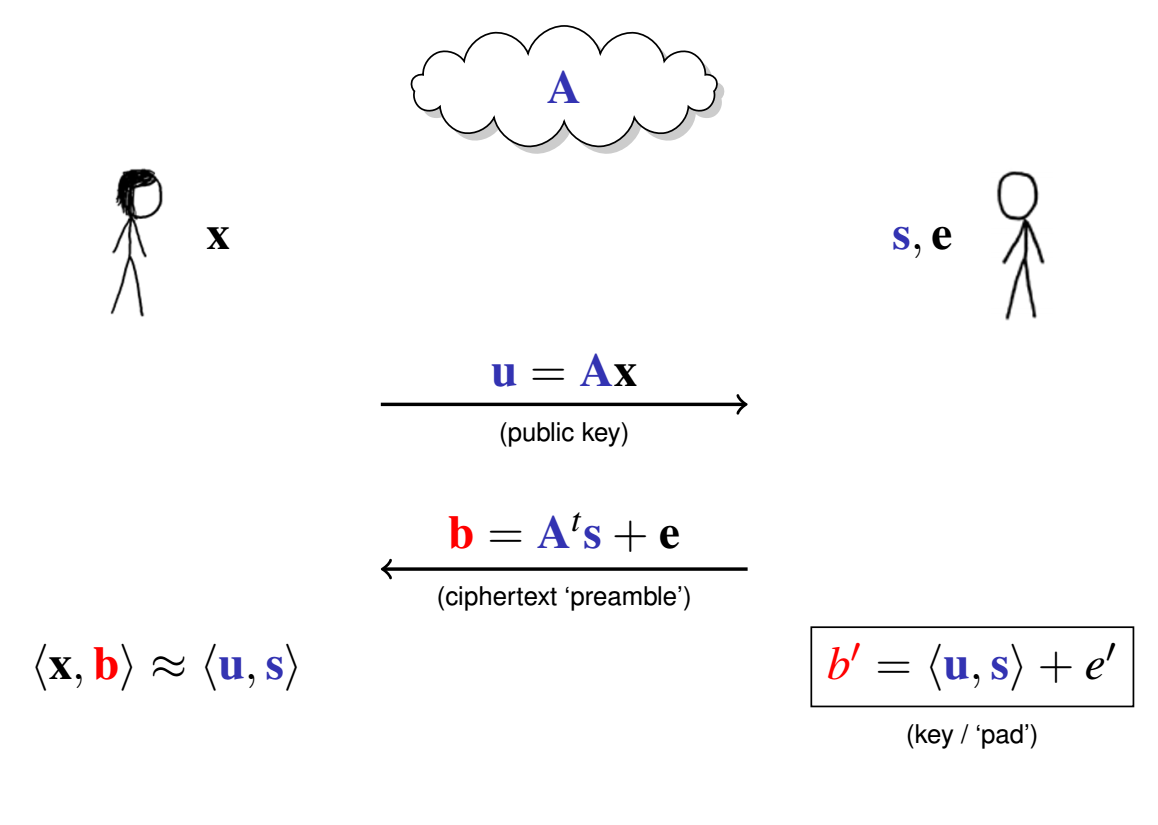
\includegraphics[width=0.3\textwidth]{LatticeBasedCryptography.png}
\caption{Lattice based Cryptography}
\end{figure}

From the above given figure 2, Alice and Bob share a public matrix $A$ where $x$ is the private vector for Alice. Alice sends $u$ vector which is the collision resistant hash function and is the product of the public matrix $A$ and Alice’s private vector x and so $u = Ax$.Now, Bob has random vectors $b$ and $b'$ where he adds his error terms $e,s$ which are random vectors and sends it Alice such that $b= As+ e$ and $b' = su + e'$.Inorder to make sure that the message sent to Alice is by bob and is not intruded by anyone, the decryption techniques is used where a parity error bit of $q/2$ is added to $b'$ which makes it $b'= su +e'+q/2$  bits. When Alice receives it, she multiplies her private vectors with $b$ and $b'$ and checks whether the value of $(x, b)$ is closer to the value of $(u, s)$ which ensures that there has not been any intrusion. If the values were not closer then it is notable that there has been an intruder \cite{crockett2016}.

Similarly, all the other approaches can also be practically applied in lattice based cryptography for enhancing the security of post quantum cryptography. As of now, for the 128 bits security in NTRU the recommended public key is represented as a degree 613 polynomial having a coefficient of mod $2^10$ which gives to a public key size of 6130 bits for which the corresponding private key would be 6743.Further works are being carried out to reduce the key size to increase the efficiency \cite{aysu2013}. 


\section{Symmetric Key Cryptography}
\subsection{Symmetric Key Cryptography in Quantum Computing Age}
\noindent Although most of asymmetric primitives are vulnerable against quantum computing, symmetric primitives seem less affected by the presence of large scale quantum computers in future. This is because the quantum algorithm works on symmetric key cryptography is based on Grover’s algorithm, which is not as shockingly fast as Shor’s algorithm \cite{bernstein2009}.  Grover’s algorithm \cite{grover1996} provides only a quadratic speed-up for exhaustive key search in classical computers. It is believed that this weakness can be compensated by doubling the key size in the design. 

Except for exhaustive search, the security of symmetric cipher is also related to cryptanalysis. Several research activities have been carried out to study the quantum attacks based on classical cryptanalytic attacks. In particular, a quantum distinguishing attack presented in \cite{kuwakado2010} is able to attack three-round Feistel. This attack is based on the quantum algorithm of Simon \cite{simon1997}. Similarly, this algorithm is extended to obtain a quantum related-key attack in \cite{roetteler2015} and a slide attack to break the block cipher operation modes for MACs \cite{kaplan2016}. Recently, Kaplan et al. \cite{kaplan2015} analysed the quantum version of differential attack on LAC, KLEIN-64 and KLEIN-96 and concluded that quantizing the best known classical differential attacks may not give the best quantum attack. All these works show that it is necessary to conduct more comprehensive study of how quantum cryptanalysis can affect the security of symmetric ciphers. However, in contrast to public-key cryptography, symmetric cryptographic algorithms are not collapsed against quantum attacks. Therefore, it is more desirable to exploit symmetric primitives when consider the security of IoT, especially for resource constrained IoT devices. 

\subsection{Authentication in RFID based IoT}
\noindent In this report, we focus on the authentication problem in IoT. More precisely, we consider the Radio Frequency Identification (RFID) based IoT applications. For instance, RFID is widely used in ticketing. It is embedded in tickets or wristbands and can be used as access to events and festivals. However, possible threats exist in this application. The legitimate RFID tag may be impersonated or a malicious party may replay the data intercepted from former transmission. In order to tackle these security issues, an efficient authentication scheme is a necessity.  In the past years, many authentication schemes for resource constrained IoT devices have been proposed. There are mainly two components considered in these designs including underling cryptographic primitives and the series of message exchanges. 

Due to the fact that RFID tags have limits on power, area and latency, lightweight cryptography tends to be more suitable than traditional cryptography. Many light-weight asymmetric and symmetric primitives such as ECC, AES, PRESENT, WG-7 and hash functions have been exploited in literature. For RFID applications, the best choice of underlying cryptographic primitive should be the one that guarantees optimum level of efficiency and security in practice.

We compare the hardware performance of three typical algorithms in Table 1. This implementation result is partial of Sghaier’s work \cite{sghaier2017}. They implemented FPGA designs in VHDL and computed several hardware performance metrics including area, frequency and power consumption. 

\begin{table}[ht]
\centering
\caption{Comparison of Hardware Performance}
\label{Table.1}
\begin{tabular}{ |p{2.5cm}|p{1cm}|p{1.5cm}|p{1cm}|  }
 \hline
 \multicolumn{4}{|c|}{FPGA Implementation} \\
 \hline
 Cryptographic Primitives & Area (Slices) & Frequency (MHz) & Power (mW)\\[0.5ex] 
 \hline 
 ECC   & 9670    &147.5&   45\\
 SHA-256 &   1480  & 73   &50\\
 Grain-128 &495 & 238.5&  19.22\\
 \hline
\end{tabular}
\end{table}

It is obvious that symmetric primitives are more efficient than asymmetric primitives in hardware implementation. We then compare the hardware performance between different symmetric algorithms. Table 2 shows the results of comparison between AES-128, SHA-1, SHA-256, Grain and Trivium from \cite{kitsos2008}. Table 3 shows the results of comparison between Trivium, Grain-128 and Mickey 128 from \cite{good2007}.

\begin{table}[ht]
\centering
\caption{Comparison of Hardware Performance}
\label{Table.2}
\begin{tabular}{ |p{2.4cm}|p{1.2cm}|p{1.2cm}|p{1.2cm}|  }
 \hline
 Cryptographic Primitives & Security (bits) & $I_{mean}$ (\mu A) & Chip Area (GE)\\[0.5ex] 
 \hline 
 AES-128   & 128    & 3.0 &   3400\\
 SHA-256 &  128  & 5.86   & 10868\\
 SHA-1 & 80  & 3.93 & 8120\\
 Grain & 80 & 0.8 &  3360\\
 Trivium & 80 & 0.68 & 3091\\
 \hline
\end{tabular}
\end{table}

\begin{table}[ht]
\centering
\caption{Comparison of Hardware Performance}
\label{Table.3}
\begin{tabular}{ |p{2.4cm}|p{1cm}|p{1.6cm}|p{1.2cm}|  }
 \hline
 Cryptographic Primitives & Key (bits) & Clock Frequency (MHz) & Area (GE)\\[0.5ex] 
 \hline 
 Trivium &  80  & 358.4   & 2599\\
 Grain-128   & 128    & 925.9 &   1857\\
 Mickey & 128  & 413.2 & 5039\\
 \hline
\end{tabular}
\end{table}

We can conclude from the above tables that stream cipher requires the lowest hardware footprint. More discussion include the quantum computing
As another direction, the security of these candidates should also be taken serious consideration. We compare the existing work of cryptanalysis of Grain family ciphers because they are well studied. The result is presented in Table 4. The symbol '$\surd$' means that the attack is successfully amounted on the cipher, while '-' denotes resistance to the attack.

\begin{table*}[t]
\centering
\caption{Comparison of Security between Grain Family Ciphers}
\label{Table.4}
\begin{tabular}{ |p{2.4cm}|p{1cm}|p{1.5cm}|p{1.5cm}|p{1.3cm}|p{1.2cm}|p{1.2cm}|p{1.5cm}|  }
 \hline
 Cryptographic Primitives & Key (bits) & Internal States (NLFSR + LFSR) & Distingui-shing Attack & Key Recovery Attack & Time-Memory-Data Trade-Off Attack & Chosen IV Attack & Guess and Determine Attack\\[0.5ex] 
 \hline 
 Grain v0 &  80  & 80 + 80   & $\surd$ & $\surd$ & $\surd$ & $\surd$ & -\\[0.5ex]
 Grain v1 &  80  & 80 + 80   & - & - & $\surd$ & - & -\\[0.5ex]
 Grain-128 & 128 & 128 + 128 & $\surd$ & - & - & $\surd$ & -\\[0.5ex]
 Grain-128a & 128 & 128 + 128 & - & - & - & - & -\\[0.5ex]
 \hline
\end{tabular}
\end{table*}

To date, there is no valid attack that has been successfully mounted on Grain-128a, which means it is the most promising underlying cryptographic primitive for authentication schemes in RFID based IoT environment.

Regarding the series of message exchanges, we study the OSK family of authentication schemes and the PFP family schemes. OSK \cite{ohkubo2003} is the first identification protocol aims at providing forward privacy and its variants \cite{ohkubo2004, avoine2005} have been proposed and presented as authentication protocols. Note that these protocols are based on hash functions and their efficiency stands out among the privacy-friendly authentication schemes compared in \cite{avoine2013}. However, the OSK family protocols have desynchronization issues and traceability weakness. An alternative authentication scheme called PFP is proposed in \cite{berbain2009} to provide stronger forward privacy and its variant PEPS \cite{billet2010} is proposed to accommodate stream cipher. The execution process is shown in Figure 3. First, the Reader initiate a challenge by sending $n/2$-bit message $a$ to the tag. After receiving the challenge, the tag combine it with a randomly generated number $b$ which is also $n/2$-bit. Then initiate the stream cipher with $a||b$ and its current key $K$ and responds with first $l$-bit output sequence $c=G_t(a||b,K)$. The reader searches for the right key $K'$ to generate the same output as $c$. Then it sends the subsequent $l$-bit message $d=G_r(a||b,K')$ to the tag. At the receipt of $d$, the tag check the validity of $d$. If the validation passed, it replace the current key $K$ with subsequent $k$-bit sequence $G_s(a||b,K)$, and the reader also update the information for this tag as $(K',G_s(a||b,K')$. The authentication is completed.

\begin{figure}[H]
\centering
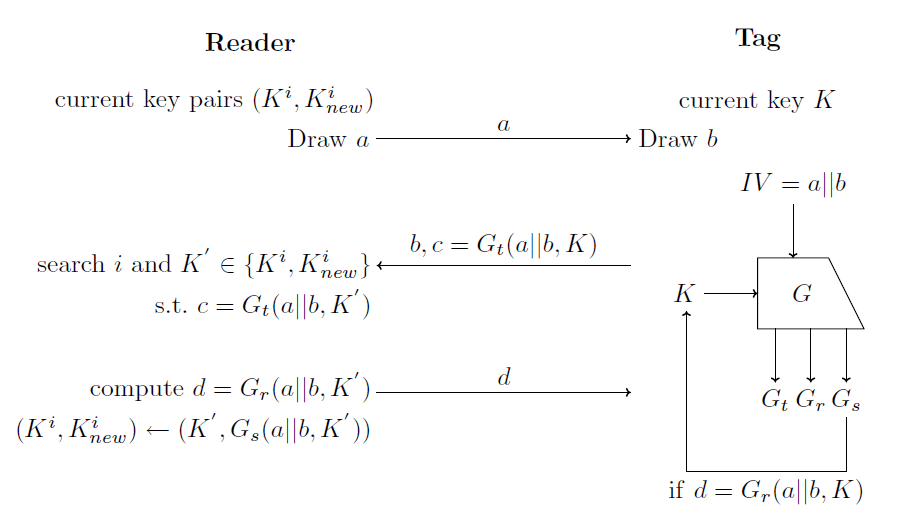
\includegraphics[width=0.5\textwidth]{PEPS.png}
\caption{ PEPS Protocol}
\end{figure}

The PEPS protocol contains only three message exchanges while provides strong forward privacy and DoS-resistance. More importantly, it is suitable for arbitrary secure stream cipher. Combing the Grain-128a stream cipher with this protocol, we can obtain a very efficient and secure authentication scheme for the RFID absed IoT system.

\section{Conclusion}
In this report, we introduce the IoT development and application status and discuss the security problem of resource constrained devices. Considering the upcoming quantum computing era, we compare the state-of-art post quantum cryptography and focus on the lattice based cryptography and symmetric cryptography. The underlying mathematical problems and an encryption/decryption process of lattice based cryptography are presented in details. Besides, we study the authentication problem of RFID devices. By comparing the hardware performance and security of existing lightweight cryptogaphy. We conclude that Grain-128a is the most promising building block for RFID based IoT environment. The PEPS is also identified as the most efficient protocols that accommodates stream cipher. The combination of these two candidates achieves an efficient and secure authentication scheme.  

%% The Appendices part is started with the command \appendix;
%% appendix sections are then done as normal sections



%% References
%%
%% Following citation commands can be used in the body text:
%% Usage of \cite is as follows:
%%   \cite{key}         ==>>  [#]
%%   \cite[chap. 2]{key} ==>> [#, chap. 2]
%%

%% References with bibTeX database:

\bibliographystyle{elsarticle-num}
%\bibliographystyle{elsarticle-harv}
% \bibliographystyle{elsarticle-num-names}
% \bibliographystyle{model1a-num-names}
% \bibliographystyle{model1b-num-names}
% \bibliographystyle{model1c-num-names}
% \bibliographystyle{model1-num-names}
% \bibliographystyle{model2-names}
% \bibliographystyle{model3a-num-names}
% \bibliographystyle{model3-num-names}
% \bibliographystyle{model4-names}
% \bibliographystyle{model5-names}
% \bibliographystyle{model6-num-names}

\bibliography{sample}

\end{document}

%%
%% End of file `elsarticle-template-num.tex'.
